\title{Distributed Computing III}
\author{Richard Thomas}
\date{\week{9}}

\maketitle

\section{Introduction}

In our introduction to distributed systems we described the fallacies of distributed systems \cite{distributed1-notes}.
Some of these fallacies (e.g. the network is reliable, the network is secure and the topology never changes)
apply Murphy's Law, \textit{if anything can go wrong it will}, to the context of distributed systems.
We will now move on to O'Toole's Commentary, \textit{Murphy was an optimist}.

Large distributed systems may consist of hundreds or thousands of computing platforms,
communicating over large distances and using unreliable internet connections.
Failure of some part of the system is practically guaranteed \cite{datacenter-computer},
the system must be designed to cater for \emph{partial failure}.
Even for small systems, some part will eventually fail,
so fault handling must be part of the design.


\section{Fault Handling}\label{sec:faults}

We mentioned that, paradoxically, distributed systems can be more reliable than non-distributed systems
because a distributed system spreads risk of failure over multiple machines \cite{distributed1-notes}.
This is managed through health checks, load-balancing and auto-scaling.
We also described the use of transactions as a mechanism to deal with some potential failures
that affect storage of persistent data \cite{distributed2-notes}.

The challenge, particularly when implementing health checks, is determining when a fault has occurred.
Most distributed systems communicate over a TCP/IP network.
This introduces a layer of uncertainty in trying to determine if a fault exists.
A message sent over a TCP/IP network may not be delivered, may be delayed, or the response may not be received.
Possible causes of these faults include the following.
\begin{itemize}
    \item The request sent to another service in the system may not have been delivered.
    \item The request may be delayed and is waiting in a queue to be processed. (e.g. either the network or the service is overloaded).
    \item The node running the service may have failed.
    \item The service may be busy and has temporarily stopped responding.
    \item The service may have processed the request and replied, but it has not been received.
    \item The response may be delayed and will be received later.
\end{itemize}

\noindent
There are techniques that can be used to identify some faults, but they are not perfect.
\begin{itemize}
    \item If a compute node is running and reachable, but does not have a process listening on the destination port, the operating system should close or refuse the TCP connection. This should result in a RST or FIN packet being received by the message sender, with the caveat that the packet may be lost.
    \item If a process crashes, but the compute node is still running, a monitor program running on the node can report the failure to a health monitoring sub-system.
    \item If a router knows that an IP address is not reachable, it can reply with a destination unreachable packet. But, a router has no additional ways of knowing if an address is not reachable than the rest of the system.
    \item If the system is running on your own hardware, you may be able to query network switches to detect link failures.
\end{itemize}

\subsection{Retry and Restart}

In general, despite the techniques above, the application needs to have a strategy to detect faults
and to decide whether to retry a request or that a node is dead.
Fault handling has to be responsive in light of the uncertainty of the fault.
A general strategy is to retry sending a message a certain number of times and having a time limit.
If no response is received within the time limit the system will then decide that the node is dead,
will spin up a new node, and remove the dead node from the load balancer's list of active nodes.

The challenge with this strategy is deciding how many retry requests and how long to wait.
Multiple retries can swamp an already overloaded node, reducing its performance even more or possibly leading to it crashing.
In the first lecture on distributed systems we introduced exponential backoff as a mechanism to reduce the impact of retrying requests \cite{distributed1-slides}.
For more information about this strategy, see the retry design pattern \cite{retry-pattern}.
Simple exponential backoff can introduce peaks of load around the exponential delay.
Jitter can be added to the delay to spread out these peaks \cite{backoff-jitter}.

Determining how long to wait before deciding that a node is dead has its own challenges.
If the system decides that a node is dead,
then all clients who have sent messages to that node, and have not received a reply, will need to resend their messages to other nodes.
Waiting too long reduces the system's responsiveness, as processes wait for a the dead node to reply.
It may also reduce the system's overall performance as a backlog of requests need to be processed.

Waiting too short a time may lead to prematurely declaring a node dead.
If the node is declared dead but it is just responding slowly because of system load,
then resending messages to other nodes increases the load on other nodes.
This can lead to a cascading failure, where all nodes are overloaded to the point that they are all declared dead.
There is an additional problem of declaring a node dead, which is just slow to respond.
It will still be processing requests until it is shutdown, but those requests will be resent to other nodes.
This leads to the possibility that some actions will be performed twice.

One option to reduce the variability of message delays is to use UDP rather than TCP at the network level.
UDP does not retransmit lost packets, which helps reduces the variability of transmission time.
The drawback is that the system will need to manage more messages not being received,
as it will not have the automated retransmission of packets provided by TCP.
It depends on the type of system, which approach is more beneficial.
If the system is transmitting financial data, the greater reliability of TCP probably outweighs the reduced message delay of UDP.
Whereas a music streaming service will probably find that having less variability of delay is more beneficial than the reliability of TCP.
(Receiving an audio packet, after it needed to be played, is pointless.)

\subsubsection{Idempotency}
Retrying operations introduces a potential complication.
What happens if the receiving node received the message and processed it, but the response failed to be returned to the sender.
The sender can retry the operation, but that may have an adverse effect on the receiver if it repeats the behaviour.

One option is for each message to have an identifier.
The receiver can decide that it has already processed the message and just return the result without processing it again.
Or, if the operation will not have any adverse effect (e.g. it is a query with no side effects), it can be processed again.

The intent is that the server's state will be the same, regardless of whether it receives a message once or multiple times.
This behaviour is called the \link{idempotent consumer pattern}
{https://chrisrichardson.net/post/microservices/patterns/2020/10/16/idempotent-consumer.html}.

\subsection{Timing Faults}\label{timing}
We introduced the issue of write conflicts, when discussing multi-leader replication \cite{distributed2-notes}.
The issue of determining order of events is applicable to more than just writing to a database.
Any situation where event order is important across multiple services (e.g. message queues in an event driven architecture),
will have similar issues to overcome.

One intuitive strategy for dealing with some cases of determining event order,
is to use a timestamp to record when the event was created.
For write conflicts, the idea being that the most recent write is the correct value in the case of a write conflict.
There are two problems with this strategy.
It is likely that the clocks on the different machines will not be perfectly in sync.
It is possible that the machine on which the last write was performed has a clock that is behind the machine with the previous write.
If writes occur in close succession, it is probable that some writes will have timestamps indicating the wrong order of writes.

Trying to synchronise clocks on different computers is difficult.
Synchronising using Network Time Protocol (NTP) is not reliable.
Network transmission time means that two machines that access one NTP server at the same time
are likely to get the time result after different lengths of network delays.
The clocks on the two machines are also likely to lose or gain time at different rates after their times have been synchronised.
There is a Precision Time Protocol (PTP) that can be used for synchronisation of under a microsecond \cite{ieee-1588},
but it takes significant resources to implement.

Another problem is that computer clocks have finite precision.
Two events can occur in close enough succession, even on the same machine, that they will end up having the same timestamp.

There are a few strategies that can be applied to deal with determining the order of events, which do not rely on timestamps.
Leslie Lamport, who was referred to in the service-based architecture lecture \cite{service-based-slides},
suggested a strategy of using a logical clock to overcome issues of drift
between real clocks on different computers \cite{LamportLeslie1978Tcat}.
The key idea is that every message sent to a service includes the logical time at which it was sent.
The receiver then adjusts its logical time to be later than when the message was sent.
\textit{Designing Data Intensive Applications} describes these problems in great detail
and suggests some solution options, with their attendant tradeoffs \cite{data-intensive}.

\subsection{Byzantine Faults}\label{sec:byzantine}

Byzantine\footnote{Byzantine carries a connotation of being an excessively complicated, intrigue filled and corrupt environment.
This is probably a smear of the Byzantine Empire (\url{https://www.britannica.com/place/Byzantine-Empire}).}
faults are those that are caused by nodes that `` lie''.
Most distributed systems are implemented with the assumption that nodes are ``honest''.
An honest node is one that provides responses which the system can assume are correct.
Faults relate to the node not responding.
A lying node is one whose response may not be correct.
Two common scenarios of a lying node are, if it sends confirmation of receipt of a message but loses the message,
or if it sends contradictory data to different nodes.

\subsubsection*{Byzantine Generals Problem}
The Byzantine Generals Problem \cite{byzantine-generals} is a fictional scenario where several generals need to agree on a battle plan.
Their armies are situated in different positions, so they can only communicate by sending messengers.
These messengers can get delayed or lost (like packets in a network).

To complicate their decision making process, some of the generals may be traitors,
though most generals are loyal.
Loyal generals will only send honest messages.
Traitors may send dishonest messages or send messages disguised as coming from another general.

The problem was proposed by Leslie Lamport as an analogy of some of the extreme faults that may exist in a distributed system.
A Byzantine fault-tolerant system is one that continues to work correctly, even if some nodes are sending incorrect messages.
This may be due to errors in the node itself or in the network connection.
Data may be corrupted in storage or in transit, it may also be intercepted or spoofed by malicious attackers.

Most systems do not attempt to be Byzantine fault-tolerant, as the cost is often too high for the potential hazard.
Stakeholders need to decide if the cost is warranted for a particular system.
Flight control systems need to be Byazntine fault-tolerant.
There are enough airplanes in the air at any one time that
\link{cosmic ray bit flipping}{https://www.scienceabc.com/innovation/what-are-bit-flips-and-how-are-spacecraft-protected-from-them.html}
is guaranteed to happen.
The control systems need to deal with potentially critical sensor data being corrupted.
Blockchain protocols are designed to allow mutually distrusting parties to agree on the result of a transaction.
A blockchain network needs to assume that a hacker could breach the network.

Not catering for Byzantine faults does not mean that a system design should assume that all messages are correct.
Simple error detection (e.g. checksums) should be used to catch corrupted data.
Any user input should be sanitised before it is used as data in the system.
These strategies do not handle subtler data corruption or persistent malicious attack,
but they catch errors that should not propagate into the rest of the system.


\section{Consistency}
Consistency is the simple idea that different parts of a system agree on the same value for a data element.
Implementing consistency is much more complex than the idea, due to many of the faults that are described in section \ref{sec:faults}.

\subsection{Eventual Consistency}

Eventual consistency is a \emph{weak} guarantee.
What it guarantees is that all replicated versions of the database will eventually have consistent values for all data they store.
The issue is the time it takes to synchronise data.
It provides no guarantee of how long until reading a specific value from all replicated databases will return the same value.
A read that occurs after a write, but which reads from a replica that has not been updated, will retrieve the old (\emph{stale}) value.

\begin{figure}[h!]
    \centering
    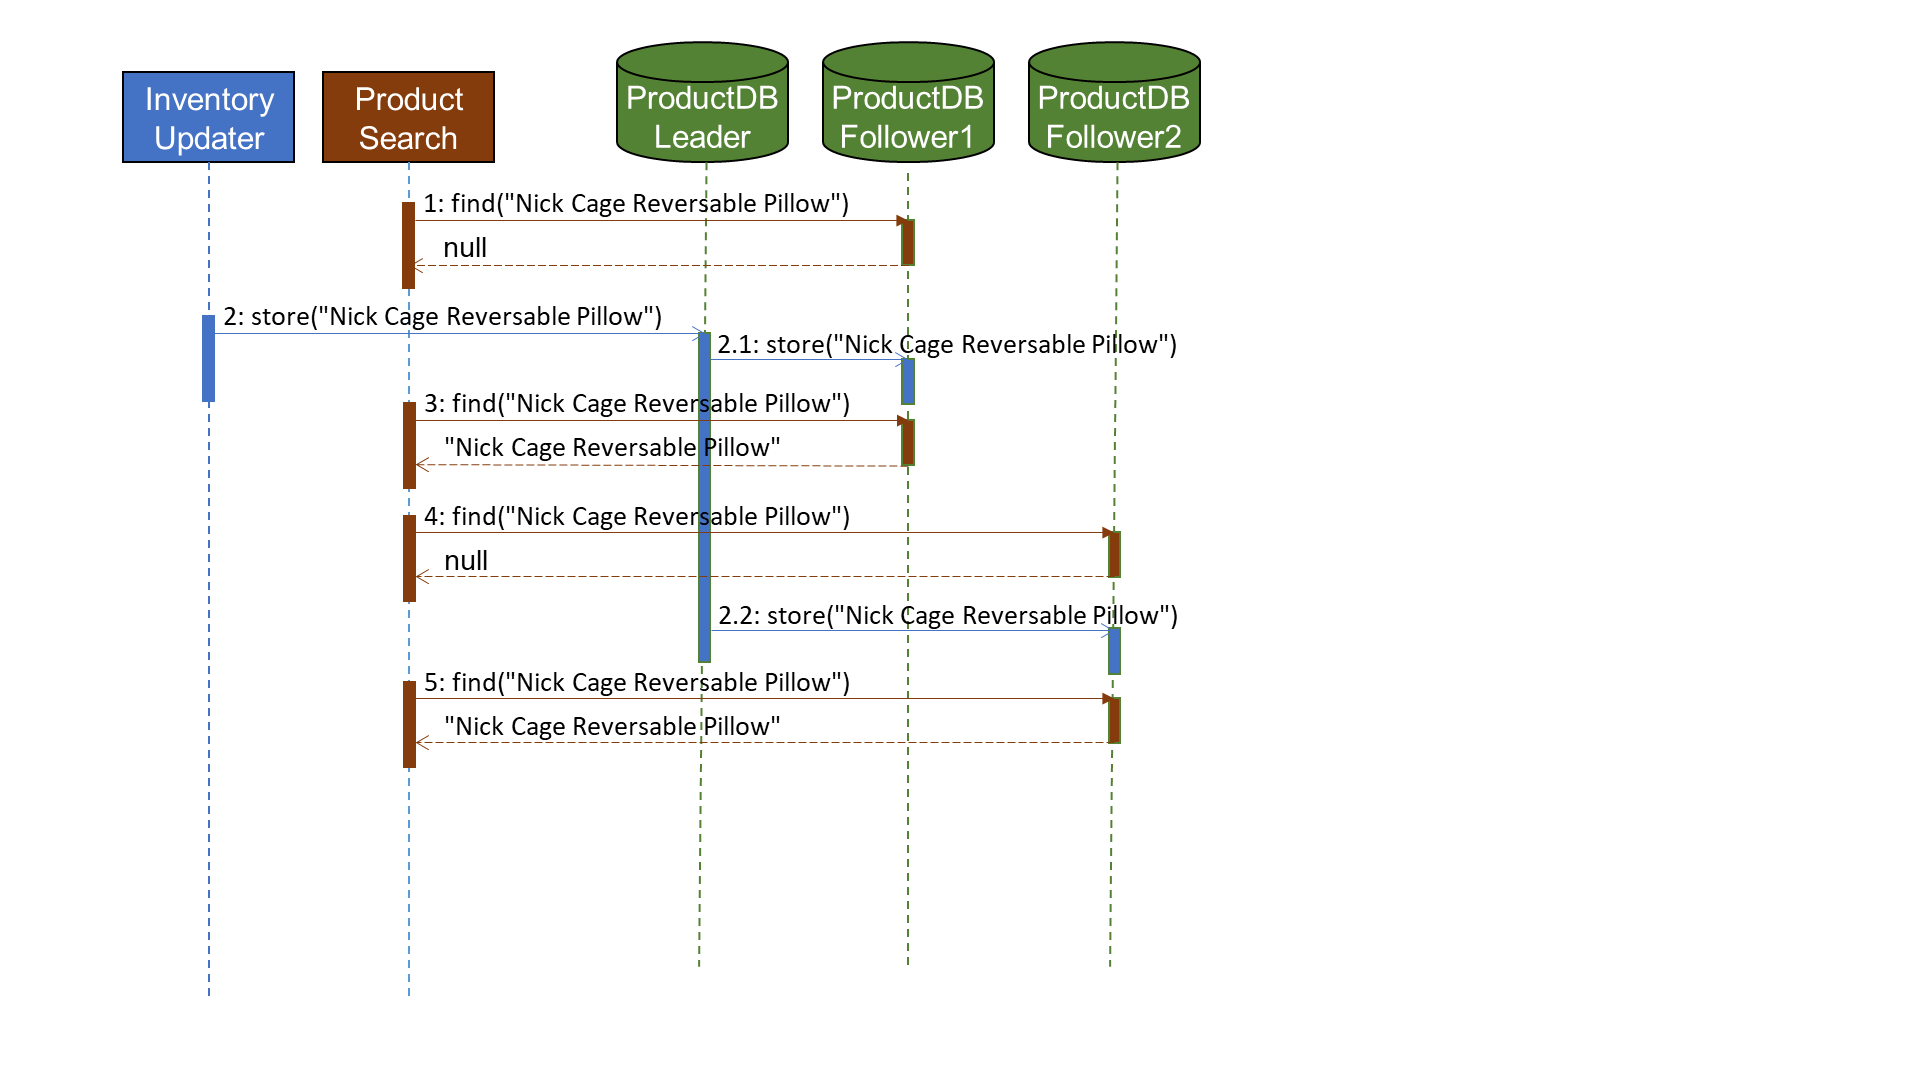
\includegraphics[trim=60 152 330 18,clip,width=0.7\textwidth]{diagrams/eventual-consistency-seq.png}
    \caption{Eventual consistency issues.}
    \label{fig:eventual-consistency-seq}
\end{figure}

Figure \ref{fig:eventual-consistency-seq} demonstrates the synchronisation issue
with an example of searching for a ``Nick Cage reversable pillow'' from the Sahara on-line store.
The product database is replicated to two followers.
Searches started after the product has been added to the store may still return that it is not available,
until all replicas have been updated.

This leads to the potential for subtle errors in the system logic.
It is difficult to think about the consequences of retrieving stale data,
as most programmers' intuition is based on the experience of modifying a value and always retrieving the new value.
The system design needs to take into account that \emph{all} database reads are performed under the assumption that the value may be stale.
Testing for errors caused by data not being consistent is difficult, as you have to force data inconsistencies.

\newpage
\subsection{Linearisability}

Contrary to eventual consistency, linearisability is a \emph{strong} guarantee.
A database system that implements linearisability provides an abstraction layer
that allows clients who use the database to work as if there is only a single instance of the database,
regardless of how many replicas have been deployed.
This provides a simple interaction model that corresponds to expectations from non-distributed systems.

Linearisability means that once a client has written data to the database,
all clients who read the that data will see the same value, regardless of the replica from which they read the data.
The challenge is implementing linearisability.

\subsubsection{Application}

Situations where linearisability can be useful include when uniqueness needs to be guaranteed.
For example, when a customer registers as a member of the Sahara eCommerce system,
they need a unique identifier.
If two people attempt to register at the same time and select the same user id,
the system needs to be able to linearise the requests to return an error message to one of the users.
The same issue arises in banking applications.
If a user transfers money from their account at the same time as an automated payment occurs,
the account debit service may need to guarantee that the account balance does not become negative.
It needs to be able to linearise these two operations and disallow one if it would result in a negative balance.

In some situations, it is acceptable to not require linearisability of operations.
If two customers order the last item of a product in the Sahara eCommerce system,
the stakeholders and designers may decide that they will allow both orders to proceed.
The resolution may be that when the fulfillment service or the warehouse discover that
the product is out of stock, they generate an event that changes one of the customers' orders to become a backorder.

The simplistic implementation of linearisability is to have a single database.
This defeats the purpose of replicating a database to improve performance and reliability.

\subsubsection{Single-Leader Replication}\label{sec:slr}
Single-leader replication can be implemented in such a way as to provide linearisability.
This is implemented by only allowing reads to be from the leader or from followers that are synchronously updated by the leader.
This means that the replicated databases can guarantee that all reads after a write will return the current value.

Forcing all reads to be from the leader defeats one of the purposes of replicating a database,
which is the performance benefit of performing queries on followers and only using the leader for update operations.
Synchronous updates of at least some followers defeats the performance benefit of asynchronous communication,
but at least allows queries on followers.
Either of these approaches maintain the reliability advantage of replicating the database.

An additional complication to implementing linearisable single-leader replication is determining which replica is the leader.
A typical approach is to have a lock of some form that is acquired by the leader, and all other replicas are followers.
Acquiring the lock itself must be a linearisable operation.
If more than one replica believes it is the leader, it means that write behaviour cannot be linearisable.
A coordination service, such as \link{etcd}{https://etcd.io/}, can be used to implement distributed locks in a linearisable fashion.

\subsubsection{Multi-Leader Replication}
Multi-leader replication cannot provide linearisability,
without introducing so many constraints as to eliminate any benefit of using the approach in the first place.
This is because multi-leader replication allows concurrent writes to multiple leaders,
and the data is asynchronously replicated to the followers and other leaders.

\subsubsection{Leaderless Replication}
It is difficult to provide linearisability with leaderless replication.
Quorum reads \cite{distributed2-notes} do not guarantee linearisability.
With asynchronous communication and network delays it is possible for a write to start,
but for a concurrent read to obtain stale data from all members of the quorum that were queried.
This occurs when a read retrieves a value from a database that has not yet been written to,
but after the write operation started and other databases were updated.
The read obtains a consistently stale value, despite obtaining the data from a quorum of databases.

It is possible to provide linearisability using strict quorums with leaderless replication.
This comes at the cost of performance, just as it does with single-leader replication.
Writes must read the state of a quorum of databases and obtain a lock on the value before performing the write.
This allows the write to be performed synchronously.

In leaderless replication, only basic read and write operations are linearisable.
More sophisticated atomic operations or transactions require a consensus algorithm to be used to provide linearisability.

\subsubsection{Consensus Algorithms}
Consensus algorithms, which will be described in section \ref{sec:consensus}, have some similarity to single-leader replication.
Their internal implementations prevent stale replica data or having multiple leader nodes.
The previously mentioned coordination service, etcd, implements its own consensus algorithm,
that provides a key-value store that guarantees linearisability.

\subsubsection{Consequences}
Linearisability means that if some database replicas lose network connection to the rest of the system,
they cannot process any requests.
Writes cannot be made as they cannot be linearised.
Reads connot be made as they may obtain stale data.

Consequently, systems, or parts of systems, that require linearisability demonstrate lower availability due to potential network faults.
This observation is known as the CAP theorem \cite{BrewerE2012Ctyl}.
Distributed systems can have \emph{consistency} in the presence of network \emph{partitioning}.
Or, they can have \emph{availability} in the presence of network \emph{partitioning}.
The ideas have been around since the mid 1970's \cite{rfc677}, despite the much more recent reference to the CAP theorem.
The prime value of the CAP theorem is how it influenced the development of NoSQL databases.

\subsection{Causal Ordering}\label{sec:causal-order}

Linearisability is one approach to defining the order in which read and write operations are conceptually performed.
It defines a \link{total order}{https://mathworld.wolfram.com/TotallyOrderedSet.html} on the operations.
This means that operations can be compared to each other to determine which should be considered to have occurred first.
Or, from the perspective of the linearisability abstraction, there are no concurrent operations on the database.

Another approach to defining the order of operations is to define a \emph{partial} order based on causality.
That is the ordering is based on one operation occurring before another (i.e. they are causally related),
but other operations may be concurrent.
A Git repository's history demonstrates causal dependencies.
Within a single branch commits occur in sequential order.
But, with multiple branches, development on each branch progresses in parallel with the others
and commits may occur concurrently on different branches.

Causal ordering is not as strict as linearisability, which in turn results in less performance cost to implement causal ordering.
The issue is to capture causal dependencies.
This requires a mechanism to determine which operation happened before another one.
The consequence is that the operations must be performed in the same order on all replicas.
If causal ordering is not required for some operations, they may occur concurrently
and it does not matter if they execute in a different order on a replica.

A single-leader replicated database can record an increasing sequence number with every write operation it records in its log.
Followers can then read the log to execute writes in sequence number order.
All followers will then be causally consistent with the leader.
The drawback is that a single-leader cannot be scaled if asynchronous writes occur faster than it can process them.
There is also the difficulty of handling the situation where the leader fails and selecting a new leader.

\subsubsection{Lamport Timestamps}
If the system does not have a single-leader, the logical clock approach mentioned in section \ref{timing} provides a mechanism to define causal ordering.
This approach is called \emph{Lamport timestamps} \cite{LamportLeslie1978Tcat}.
Each node has an id and counts the number of operations it has executed.
The timestamp is a tuple (\emph{counterValue}, \emph{nodeID}).
The \emph{nodeID} guarantees that every timestamp is unique, even if they have the same counter value.
Every node stores the \emph{maximum} counter value it has seen so far.
This maximum is passed in every request to another node.
If a node receives a request or response with a maximum counter value greater than its own counter value,
it increases its own counter to the new maximum.

\begin{figure}[h!]
    \centering
    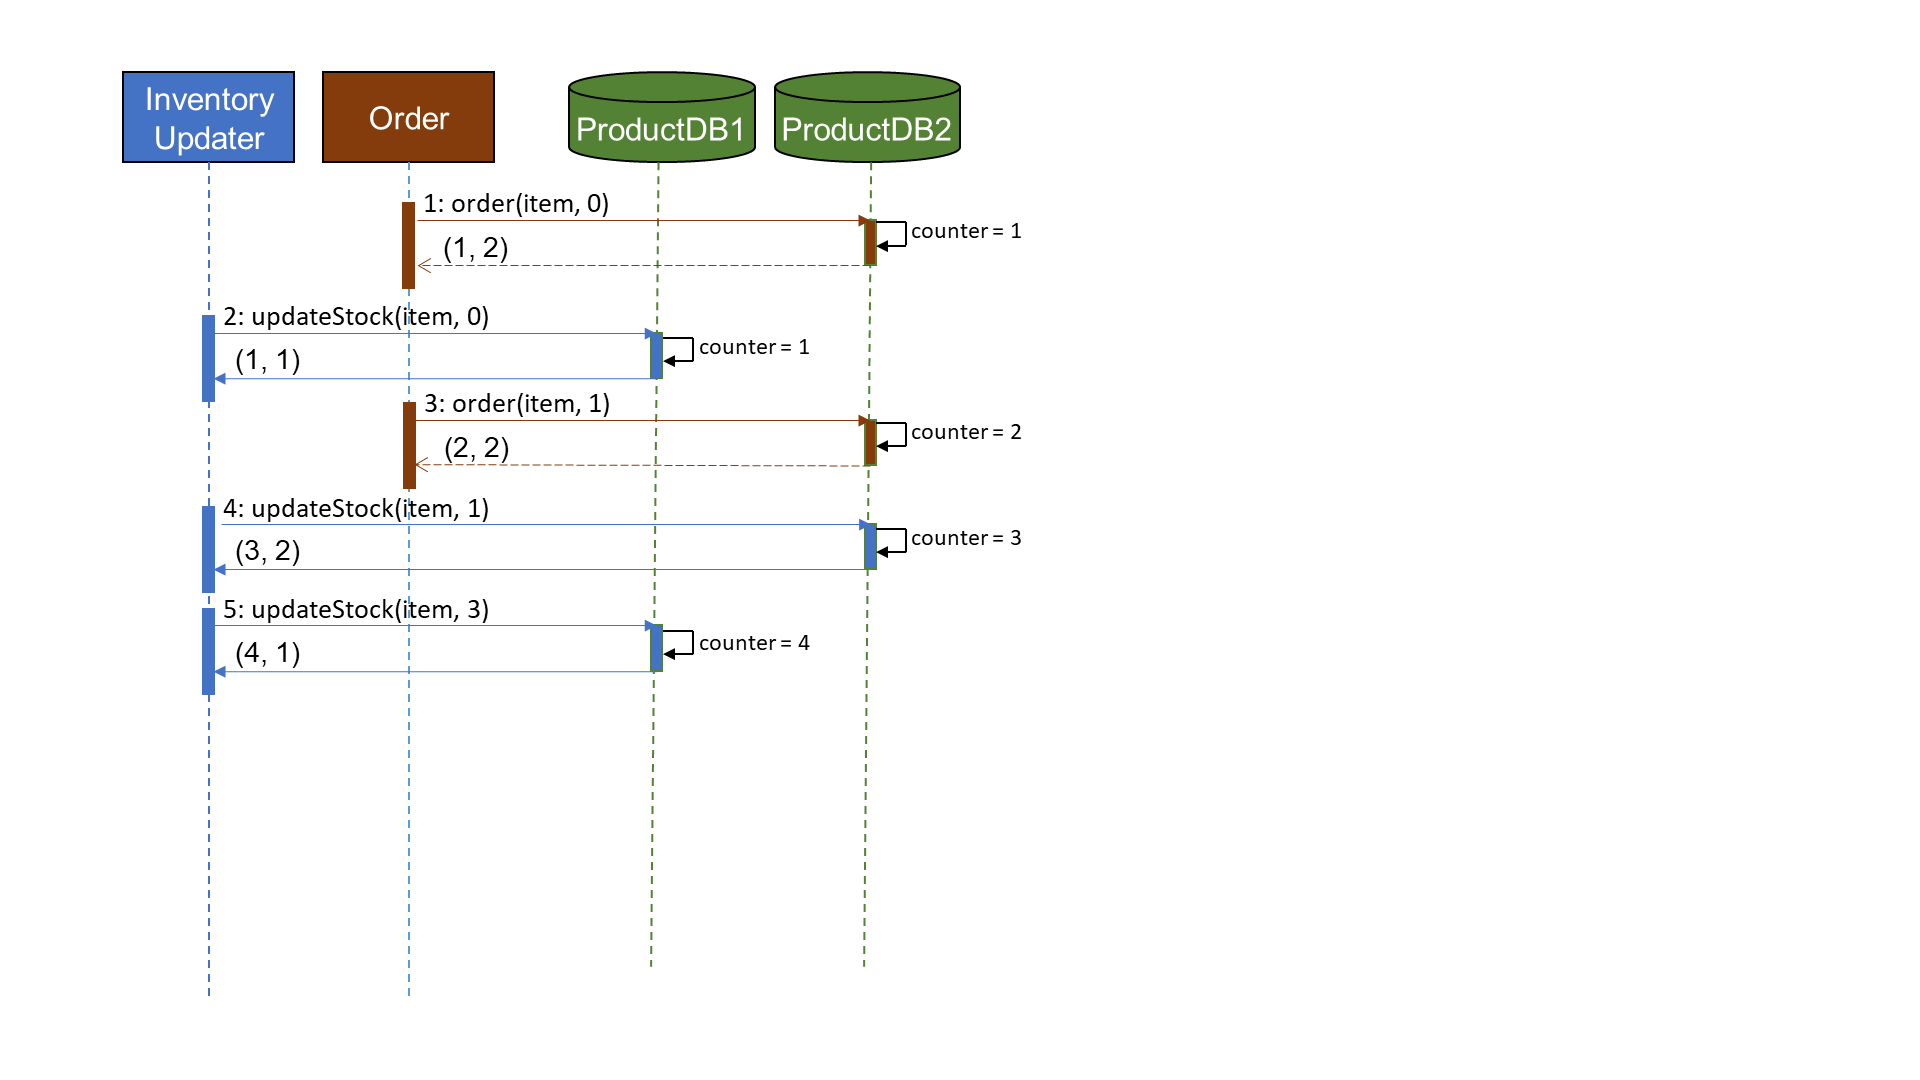
\includegraphics[trim=60 189 450 35,clip,width=0.67\textwidth]{diagrams/lamport-timestamp-seq.png}
    \caption{Lamport timestamps.}
    \label{fig:lamport-timestamp-seq}
\end{figure}

In figure \ref{fig:lamport-timestamp-seq}, when \texttt{InventoryUpdater} sends message \texttt{4} to \texttt{ProductDB2},
the message includes a parameter which is \texttt{InventoryUpdater}'s current maximum value, which is \texttt{1}.
\texttt{ProductDB2}'s counter value is already \texttt{2},
so it increases it to \texttt{3} and returns it as part of the Lamport timestamp to \texttt{InventoryUpdater}.
\texttt{InventoryUpdater} records \texttt{3} as its new maximum value.
When \texttt{InventoryUpdater} sends message \texttt{5} to \texttt{ProductDB1},
the message includes \texttt{InventoryUpdater}'s maximum value of \texttt{3}.
\texttt{ProductDB1}'s counter value was \texttt{1}, so it increases it to \texttt{4} and returns it to \texttt{InventoryUpdater}.

Lamport timestamps define causal ordering for operations, but they do not guarantee consistency when an operation is performed.
If two orders are sent to \texttt{ProductDB1} and \texttt{ProductDB2} at the same time and there is only one item in stock,
Lamport timestamps provide a way to decide which order occurred first, but only emph{after} the orders are processed.

To enforce a constraint that would not allow two orders for the last item in stock,
there needs to be a mechanism to indicate when the order is completed.
\emph{Total order broadcast} is one technique that does this.
Messages are ordered by their delivery time, not when a result is returned.
So, if a message has been received, another message cannot be performed before it.
Coordination services, such as \link{etcd}{https://etcd.io/}, implement total order broadcast.


\section{Consensus}\label{sec:consensus}

In a distributed system, consensus is when a set of nodes in the system agree on some aspect of the system's state.
Achieving consensus is a difficult problem, in light of the issues described in section \ref{sec:faults}.
When designing a distributed system, you can take advantage of the abstraction of consensus to ignore the faults it handles.
Abstractions like consensus and transactions \cite{distributed2-notes} make it easier to reason about the behaviour of a distributed system.
In this section, we will look at how consensus can be implemented.

\subsection{Consensus Algorithms}

Consensus is formally described as ``one or more nodes may \emph{propose} values,
and the consensus algorithm \emph{decides} on one of those values.''
For example, if multiple customers attempt to buy the last item that is in stock,
each node handling a customer request proposes its customer as the purchaser.
The consensus algorithm decides which customer becomes the purchaser.
A consensus algorithm must satisfy the following properties \cite{cachin2011Distributed}.

\begin{description}
    \item[Uniform Agreement] All nodes must agree on the decision.
    \item[Integrity] Nodes can only vote once.
    \item[Validity] If the decision is the value $v$, then $v$ must have been proposed by a node.
    \item[Termination] Every node that does not crash must decide on a value.
\end{description}

Uniform agreement and integrity are the keys to consensus.
All participants must agree on the same decision, and once a participant agrees they cannot change their decision.
Validity is a formal requirement to avoid nonsensical solutions (e.g. always agreeing to a null decision).
Termination enforces fault tolerance.
It requires that the consensus algorithm progresses towards a solution, and does not wait for permanently failed nodes.
It essentially is saying that if some nodes fail,
the other nodes must make a decision and reach consensus with those nodes that are still working.
Any consensus algorithm requires at least a majority of the nodes trying to achieve consensus
to remain functioning in order to assure termination \cite{chandra1996reliable}.
Most implementations of consensus algorithms ensure that uniform agreement, integrity and validity are always met, 
even if a majority of the nodes fail.
This means that even in the worst case it will not result in the consensus algorithm making an invalid decision,
it just means that it will not be able to achieve consensus and will not be able to process requests.

Some commonly used consensus algorithms are Viewstamped Replication (VSR) \cite{vsr1988},
Paxos \cite{paxos1998}, Raft \cite{raft2015}, and Zab \cite{zab2011}.
You are not expected to be able to implement a consensus algorithm, as it is very challenging to implement correctly.
You should be aware that consensus algorithms exist and then find a library or service that implements one that suits your scenario.
For performance reasons, most consensus algorithms do not directly implement the formal model described above.
They typically implement total order broadcast, as mentioned in section \ref{sec:causal-order}.
It requires that messages are delivered exactly once, and in the same order, to all nodes.
This provides a result equivalent to multiple rounds of consensus determining the order in which messages are sent.

Most consensus algorithms assume that there are no Byzantine faults, as described in section \ref{sec:byzantine}
(e.g. a node sending contradictory messages to other nodes).
It is possible to implement a consensus algorithm that can manage Byzantine faults,
as long as fewer than one-third of the nodes generate Byzantine faults \cite{byzantine-tolerance-2002}.
The details of how to do this are beyond the scope of this course.

\subsection{Distributed Transactions}

A distributed system that needs to enforce a transaction across multiple compute nodes
needs a mechanism to gain consensus between all nodes participating in the transaction, so that it can be committed.
This is called the \emph{atomic commit} problem, based on the idea of transaction atomicity from ACID \cite{distributed2-notes}.

In a database, a distributed transaction may happen when the database is partitioned and data in different partitions are part of the transaction.
It will also happen if the database has a secondary index on a different node to the primary index.
Distributed transactions may also occur where events or messages are part of the transaction.
An example of this is sending a message to a message queue, while storing data in a database.
In the Sahara eCommerce system, when an order is placed it is stored in the order table in the database
and a message is placed in the notification queue to notify the customer that the order has been successful.
Storing the order may be a transaction in only a single database partition,
but to ensure the notification message is only added to the queue if the order is successful requires a distributed transaction.

\subsubsection{Two-Phase Commit}\label{sec:2pr}
A two-phase commit algorithm is a type of consensus algorithm that solves the atomic commit problem.
As the name implies, it splits the commit into two steps.
There are better consensus algorithms, as described in section \ref{sec:consensus},
but two-phase commit is fairly simple and still commonly used.
It should be noted that a two-phase commit is a consensus algorithm
but it does not satisfy the termination property, so it is not fault tolerant.

\begin{figure}[h!]
    \centering
    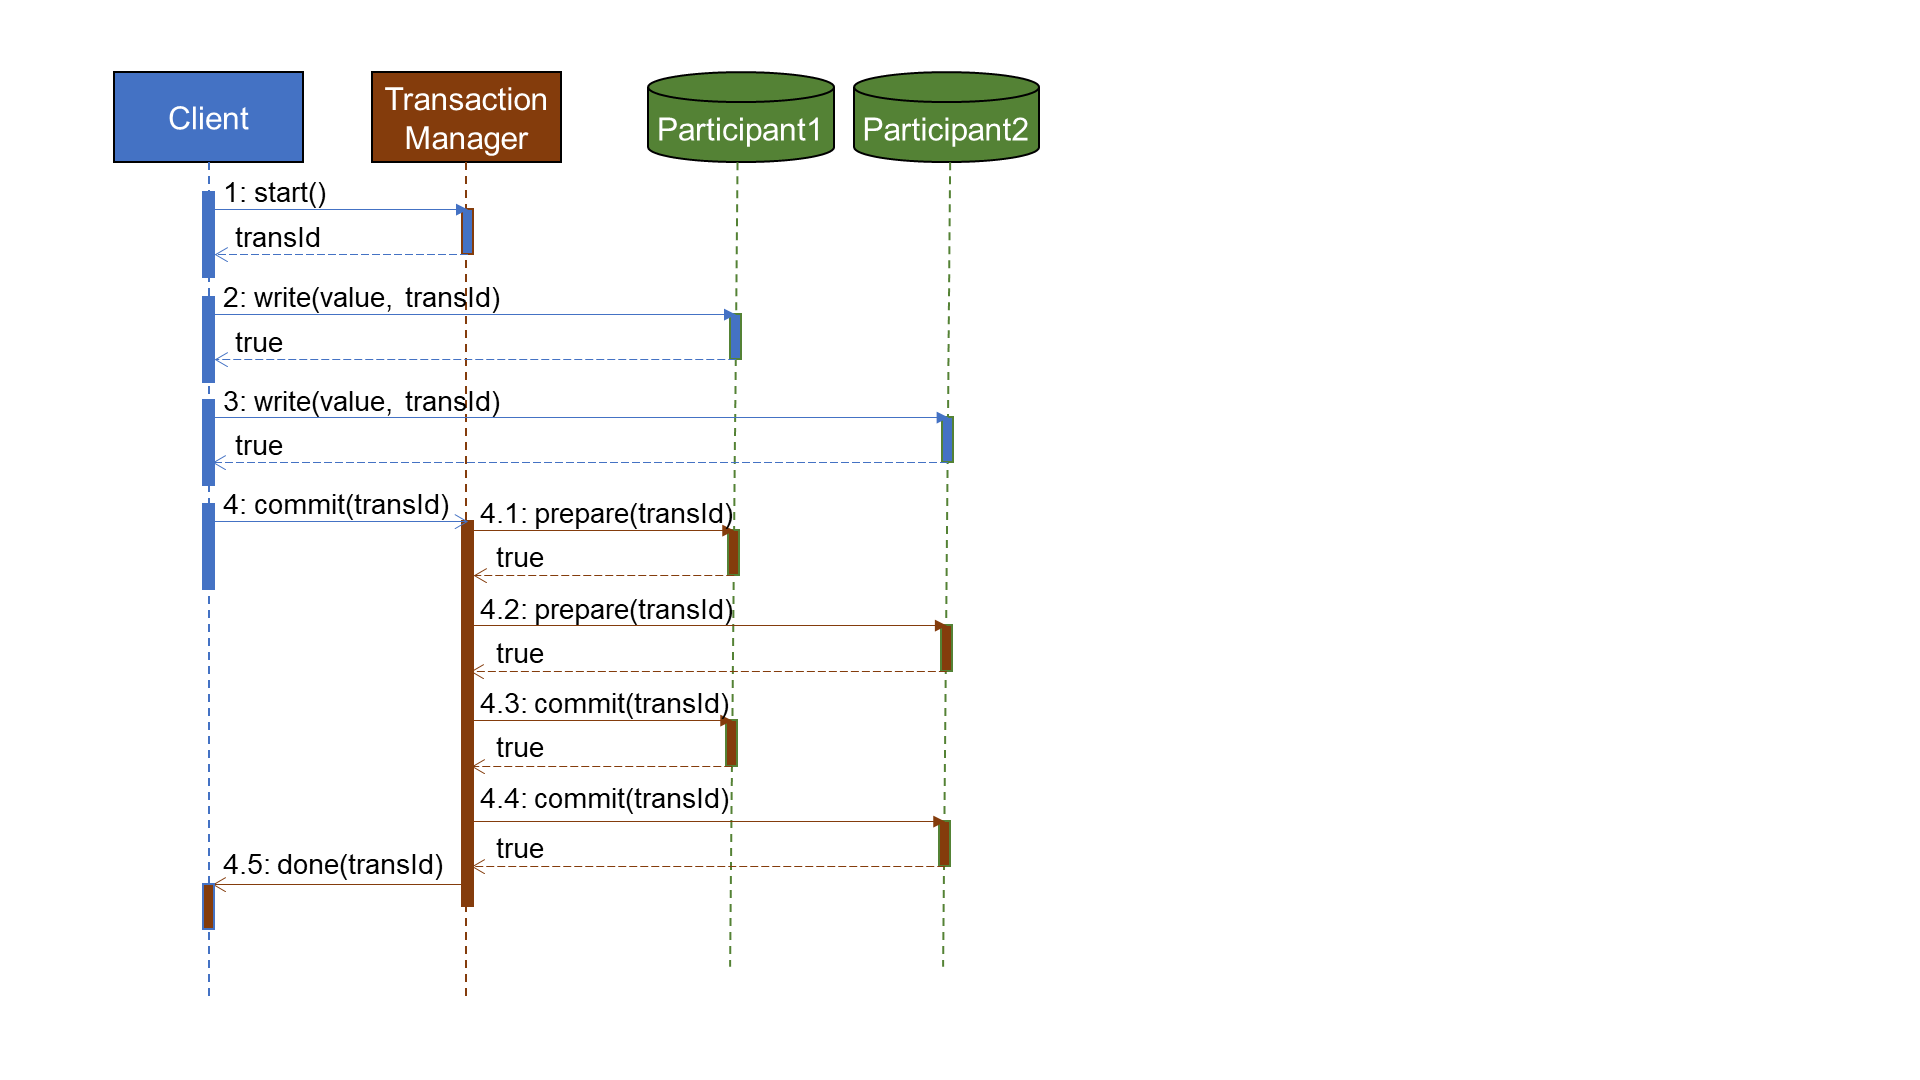
\includegraphics[trim=55 70 420 30,clip,width=0.67\textwidth]{diagrams/2phase-commit-seq.png}
    \caption{Two-phase commit.}
    \label{fig:2pc-seq}
\end{figure}

A \emph{transaction manager} is introduced to coordinate the two-phase commit process.
The database nodes that are part of the transaction are called \emph{participants}.

The process starts when some part of the system (\texttt{Client} in figure \ref{fig:2pc-seq})
requests to start a distributed transaction and receives a unique transaction identifier (\texttt{transId}).
The client starts \emph{single-node} transactions on each, attaching the \texttt{transId} to the transaction.
The client can perform multiple reads and writes as part of the transaction.

When the client is ready to commit the transaction it requests the \texttt{TransactionManager} to perform the commit.
The \texttt{TransactionManager} sends a prepare message to all the participants.
If a prepare message times out, or any participant reports a failure,
the \texttt{TransactionManager} sends an abort message to all participants and reports the failure to the client.

When a participant receives the prepare message, it confirms that it can commit the transaction,
regardless of any fault that may occur after replying to the prepare message.
(i.e. The participant has saved all changes as part of this transaction in persistent memory.)
The participant is no longer able to abort the transaction itself,
it can only abort it now if it receives an abort message from the \texttt{TransactionManager}.
In effect, it is a pseudo-commit.

When the \texttt{TransactionManager} receives positive responses from all participants,
it saves the commit decision to a persistent transaction log.
This means that even if the \texttt{TransactionManager} fails, it can recover the decision.
This is called the \emph{commit point}.
If the \texttt{TransactionManager} decides to abort the transaction,
it records the abort decision in the transaction log.

After the commit point has been reached, the \texttt{TransactionManager} sends the commit message to all participants.
This is an irreversible decision.
If the commit message fails or times out, the \texttt{TransactionManager} must continue retrying the message
until all participants report that they have committed the transaction.
This means that even if a participant crashes before it performs the commit, it will complete the commit once the participant restarts.
That was the reason for performing a pseudo-commit at the prepare stage,
if necessary, the participant can recover and redo all steps that are part of the transaction leading up to the commit.

If the \texttt{TransactionManager} fails during the commit process,
it can recover and resend the commit messages to any participant that had not responded before the \texttt{TransactionManager} failed.
If a participant had commited the transaction before the \texttt{TransactionManager} failed,
it can ignore the new commit and just report that the commit was successful.

Many libraries implement two-phase commit.
The Open Group defined the X/Open eXtended Architecture standard \cite{xa-std}, which most of these libraries follow.
Many relational databases (e.g. MySQL, Postgres, Oracle, \dots) and message queues (e.g. ActiveMQ, IBM MQ, \dots)
implement the standard.

A two-phase commit is called a \emph{blocking} atomic commit,
as completion of the commit can take a long time if a participant or the \texttt{TransactionManager} fail.
Even worse, if the transaction log on the \texttt{Transaction\-Manager} or a participant are corrupted when they fail,
this may lead to rows in the database never being unlocked.
This usually requires manual intervention to decide whether to complete the commit or roll it back, to maintain atomicity.
Some libraries that support two-phase commit can make an automated decision in this case,
but the decision will probably break atomicity.

Two-phase commit provides a simple abstraction that allows distributed systems to perform safe transactions.
The drawback is that a blocking atomic commit is a significant performance cost.
Even if the \texttt{TransactionManager}, and no participant, fails;
rows across multiple database nodes are locked until the commit completes.
If there is a failure, recovery can take a long time.
For example, in MySQL it is reported that distributed transactions are ten times slower than single-node transactions \cite{distrib-mysql}.
Consequently, most NoSQL databases and many cloud-based relational databases do not support distributed transactions.

\subsection{Leaders}

Section \ref{sec:slr} mentions issues around choosing the leader for a single-leader replicated database.
Some database systems allow the leader to be automatically elected.
This allows single-leader replication to be fault tolerant as a new leader can be elected if the leader fails.
This concept generalises to consensus algorithms, which need a leader to achieve consensus.

\emph{Epoch numbers} are used to manage this approach.
The systems guarantee that there is only one leader per epoch, rather than there only ever being one leader.
If there is no leader, or the current leader seems to be dead,
a vote is conducted amongst the nodes trying to achieve consensus to elect a new leader.
The election increments the epoch number.
Each leader has its epoch number.
If there is a conflict between leaders (e.g. a vote was conducted for a new leader when the previous leader was not dead),
the leader with the higher epoch number wins as the new leader.

Before a leader can decide on a value that has been proposed for consensus,
it checks to see if there are any other leaders with a higher epoch number.
It must obtain the results from this check from a quorum of nodes,
otherwise the check fails.


\section{Conclusion}

Designing reliable distributed systems is a complex, but manageable, process.
These notes have introduced some of the less intuitive issues that arise in distributed systems
and how to design a system to work in the presence of these issues.

It is possible to go a step further and prove the correctness of distributed systems.
This involves creating a model of the system and every service in the system.
Assumptions about system behaviour can be stated within the model.
The algorithms used to implement the system can be proven to work within the system model and its assumptions.
Of course, if the assumptions are broken, then any proofs are invalid.
\link{CSSE7610 Concurrency: Theory and Practice}{https://my.uq.edu.au/programs-courses/course.html?course_code=csse7610}
provides the background knowledge required to perform these proofs
and introduces some of the initial modelling techniques required for distributed systems.
